\documentclass[fontsize=11pt, paper=a4, DIV=9]{standalone}

 \usepackage[utf8]{inputenc}
 \usepackage[T1]{fontenc}

 \usepackage{lmodern}
 \usepackage{amsmath}
 \usepackage{amssymb}
 \usepackage{relsize}
 \usepackage{xparse}
 \usepackage{tikz}
 \usepackage{garamondx}
 
 
 % for stealth-like arrows in math mode
\usepackage{mathabx}
 
 \tikzset{>=stealth}

 \makeatletter

 % character used in a formal language
 % \Char{}  expands to the empty word
 % \Char{~} expands to the blank character of a Turing machine
 % \Char{#} expands to the bottom-of-stack character of a pushdown automaton
 \ExplSyntaxOn
 \NewDocumentCommand{\Char}{>{\TrimSpaces}m}
 {
   \str_case_e:nnF{\tl_to_str:n{#1}}
   {
     {    }           {\mbox{$\varepsilon$}}
     { ## }           {\mbox{\texttt{\#}}}
     { \c_tilde_str } {\mbox{\textscale{.87}{$\Box$}}}
   }
   {\mbox{\texttt{#1}}}
 }
 \ExplSyntaxOff

 % state of an automaton
 \newcommand{\State}[1]{#1}

 % graph of a Turing machine
 \newenvironment{GraphTM}[1][]{\begin{scope}[#1]}{\end{scope}}

 % state in a graph of a Turing machine
 % #1 = identifier 
 % #2 = state label
 % #3 = "initial" and/or "accepting" (separated by comma)
 % #4 = position in the format "(<x>, <y>)"
 \NewDocumentCommand{\StateTM}{ r() m O{} r() }{%
   \node [state, #3] at (#4) (#1) {$\State{#2}$};}

 % transition in a graph of a Turing machine
 % #1 = identifier of the current state
 % #2 = edge modifier using TikZ syntax
 % #3 = identifier of the subsequent state
 % #4 = position of the edge label using TikZ syntax
 % #5 = edge label
 \NewDocumentCommand{\TransTM}{ r() O{} r() O{} m  }{%
   \path [trans] (#1) edge [#2] node [#4] {\IT@TM@Edge@Label{#5}} (#3);}

 % internal commands used by \TransTM
 \newcommand{\IT@TM@Trans}[3]{%
   \makebox[.6em]{\Char{#1}}\;:\;\makebox[.6em]{\Char{#2}}\;,\,\Char{#3}}
 \NewDocumentCommand{\IT@TM@Edge@Item}{>{\SplitArgument{2}{,}}m}{%
   \IT@TM@Edge@Delim\IT@TM@Trans#1}
 \NewDocumentCommand{\IT@TM@Edge@Label}{>{\SplitList{|}}m}{%
   \def\IT@TM@Edge@Delim{\gdef\IT@TM@Edge@Delim{\\}}
   \shortstack{\ProcessList{#1}{\IT@TM@Edge@Item}}}

 \makeatother

 \usetikzlibrary{automata}

 \tikzset{>=stealth, semithick}
 \tikzset{initial text=}
 \tikzset{state/.style={font=\small, minimum size=0pt, circle, draw}}
 \tikzset{trans/.style={font=\footnotesize, ->}}

 \begin{document}

 \begin{tikzpicture}
 \begin{GraphTM}
 % States
 \StateTM (0) {} [initial]   ( 0, 0)
 \StateTM (1) {} (1,2)
 \StateTM (2) {} (1,-2)
 \StateTM (3) {} (5,0)
 \StateTM (4) {} (4,2)
 \StateTM (5) {} (4,-2)
 \StateTM (6) {} (7,0)
 \StateTM (7) {} [accepting] (9, 0)
 % Transitions
 \TransTM (0) [] (1) [left=3pt] {1, A, $\rightarrow$}
 \TransTM (0) [] (2) [left=3pt] {0, B, $\leftarrow$}
 \TransTM (1) [] (4) [above] {~, A, $\leftarrow$}
 \TransTM (2) [] (5) [below] {~, B, $\leftarrow$}
 \TransTM (3) [] (0) [above] {A, A, $\rightarrow$}
 \TransTM (3) [] (0) [below] {B, B, $\rightarrow$}
 \TransTM (4) [] (3) [left=3pt] {1, 1, $\leftarrow$ | 0, 0, $\leftarrow$}
 \TransTM (5) [] (3) [left=3pt] {1, 1, $\leftarrow$ | 0, 0, $\leftarrow$}
 \TransTM (3) [loop right] (3) [right=-4pt] {1, 1, $\leftarrow$ | 0, 0, $\leftarrow$}
 \TransTM (4) [] (6) [right=11pt, above=3pt] {~, ~, $\rightarrow$}
 \TransTM (5) [] (6) [right=11pt, below=3pt] {~, ~, $\rightarrow$}
 \TransTM (6) [] (7) [below] {~, ~, $\leftarrow$}
 \TransTM (1) [loop above] (1) [above] {1, 1, $\rightarrow$ | 0, 0, $\rightarrow$ | A, A, $\rightarrow$ | B, B, $\rightarrow$}
 \TransTM (2) [loop below] (2) [below] {1, 1, $\rightarrow$ | 0, 0, $\rightarrow$ | A, A, $\rightarrow$ | B, B, $\rightarrow$}
 \TransTM (4) [loop above] (4) [above] {A, A, $\leftarrow$ | B, B, $\leftarrow$}
 \TransTM (5) [loop below] (5) [below] {A, A, $\leftarrow$ | B, B, $\leftarrow$}
 \TransTM (6) [loop above] (6) [above] {A, 1, $\rightarrow$ | B, 0, $\rightarrow$}
% \TransTM (z0)                (z1) [above]    {a, x, R}         
% \TransTM (z0)                (z4) [left=3pt] {y, y, R}          
% \TransTM (z0)                (z5) [left=3pt] {~, ~, N}
% \TransTM (z1) [loop above]   (z1) [above]    {a, a, R | y, y, R}
% \TransTM (z1)                (z2) [above]    {b, y, R}
% \TransTM (z2) [loop above]   (z2) [above]    {b, b, R | z, z, R}
% \TransTM (z2)                (z3) [above]    {c, z, L}
% \TransTM (z3) [loop above]   (z3) [above]    {a, a, L | b, b, L | y, y, L | z, z, L}
% \TransTM (z3) [bend left=23] (z0) [below]    {x, x, R}
% \TransTM (z4) [loop above]   (z4) [above]    {y, y, R | z, z, R}
% \TransTM (z4)                (z5) [above]    {~, ~, N}
 \end{GraphTM}
 \end{tikzpicture}

 \end{document}